\documentclass[a4paper,11pt]{article}
\usepackage{fullpage}
\usepackage[latin1]{inputenc}
\usepackage[T1]{fontenc}
\usepackage[normalem]{ulem}
\usepackage[english]{babel}
\usepackage{listings,babel}
\usepackage{palatino}
\usepackage{gensymb}
\lstset{breaklines=true,basicstyle=\ttfamily}
\usepackage{graphicx}
\usepackage{moreverb}
\usepackage{url}
\usepackage{tabularx}
\usepackage{float}
\usepackage{tweaklist}
\renewcommand{\itemhook}{\setlength{\topsep}{0pt}\setlength{\itemsep}{0pt}}
\renewcommand{\enumhook}{\setlength{\topsep}{0pt}\setlength{\itemsep}{0pt}}

\title{SERDES-based TDC Core Test Report}
\author{S\'ebastien Bourdeauducq}
\date{July 2012}
\begin{document}
\setlength{\parindent}{0pt}
\setlength{\parskip}{5pt}
\maketitle{}
\section{The demonstration design}
\subsection{Hardware}
The demonstration design runs on a SPEC board equipped with a FMC DIO 5-channel daughterboard.

Data is transferred at 115200 8-N-1 via the serial console accessible using the built-in USB adapter. The PCIe interface is not used.

Test signals go through the FMC daughterboard. The first LEMO connector on the daughterboard is configured as output and transmits an oscillating pattern. The next two LEMO connectors are inputs connected to TDC channels.

\subsection{Contents}
The demonstration design contains:
\begin{itemize}
\item the LatticeMico32 soft processor, running at 125MHz from the clock generated by the CDCM61004 chip on the SPEC.
\item UART, timer and GPIO cores from the Milkymist SoC. Memory-mapped.
\item the TDC core with its Wishbone interface, configured for two channels, also clocked from the 125MHz source. Memory-mapped.
\item an oscillator for generating TDC test signals.
\item a basic boot ROM and command line interface based on the Milkymist BIOS.
\item software routines for testing the TDC core.
\end{itemize}

\subsection{Synthesizing and running the design}
\subsubsection{Compiling the LM32 software}
Since the LM32 software is used in block RAM initialization, it must be compiled before the FPGA bitstream is built. The scripts expect the Clang/LLVM toolchain, but any LM32 toolchain should be suitable.

You will need first to compile some host tools which are used to build block RAM initialization files:
\begin{verbatim}
cd $TDCDIR/demo/tools
make
\end{verbatim}

Then, compile the base library and the software image:
\begin{verbatim}
cd $TDCDIR/demo/software/libbase
make
cd $TDCDIR/demo/software/demo
make
\end{verbatim}

\subsubsection{Compiling the FPGA bitstream}
The design can be synthesized with ISE 14.1. The compilation is automatic:
\begin{verbatim}
cd $TDCDIR/demo/boards/spec/synthesis
make -f Makefile.xst
\end{verbatim}

\subsubsection{Downloading the FPGA bitstream}
If you are using Xilinx iMPACT, there is an automatic script:
\begin{verbatim}
cd $TDCDIR/demo/boards/spec/synthesis
make -f Makefile.xst load
\end{verbatim}

Otherwise, load the file \verb!$TDCDIR/demo/boards/spec/synthesis/build/system.bit! with your favorite FPGA programming tool.

\subsection{Command line interface}
Once the bitstream is loaded, it implements a command-line interface on the serial console (115200 8-N-1), and it displays a \textbf{TDC>} prompt. From there, you can enter the following commands:

\begin{tabularx}{\textwidth}{|l|X|}
\hline
mr <address> [length] & Reads memory. Length is in bytes (default 1). \\
\hline
mw <address> <value> [count] & Writes one or several 32-bit words to memory. Count is in words (default 1). \\
\hline
temp & Displays the current temperature in \degree C measured by the 1-wire sensor. \\
\hline
daclevel <value> & Sets the output voltage on all channels of the I2C DAC5578 digital to analog converter on the FMC DIO board. The 16-bit value is directly written into the DAC. \\
\hline
diff & In a loop, waits for a TDC event to happen in both channels, and displays its parameters. The output is in CSV format and contains the following information: polarity for the first channel, raw timestamp for the first channel, fixed-point timestamp for the first channel, and the same for the second channel. Sending any character to the console stops the series of measurements. \\
\hline
\end{tabularx}

\section{Methods and results}

\subsection{Differential measurements}
The purpose of this test is to determine the precision of the system.

We connected the oscillator output of the FMC DIO card to a splitter feeding two cables of different lengths\footnote{Those cables had propagation delays of approximately 2ns and 4ns.} going to the two TDC channels. We then observed the difference between the two TDC timestamps, which is expected to remain constant (Figure \ref{fig:dtdc}). Since the oscillator is asynchronous to the system clock, the complete delay line can be covered and tested.

\begin{figure}[H]
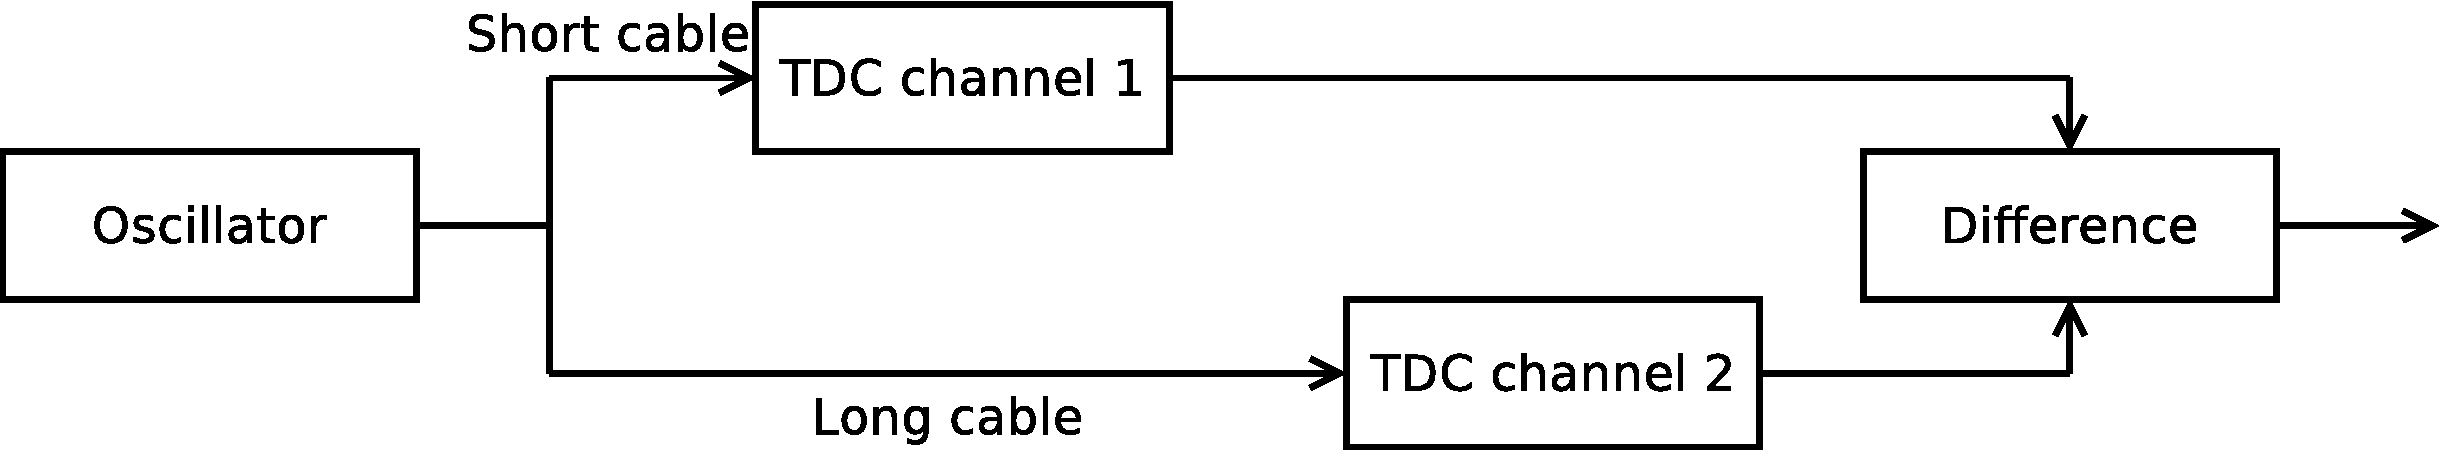
\includegraphics[width=\textwidth]{dtdc.pdf}
\caption{Principle of differential measurements.}
\label{fig:dtdc}
\end{figure}

The advantage of this technique is that it is easy to set up and does not require expensive equipment. A limitation is that the result is not affected by common-mode noise of the input path to the ISERDES.

% The histogram of the results is shown in Figure \ref{fig:mhist}.

% \begin{figure}[H]
% \includegraphics[width=\textwidth]{mhist.pdf}
% \caption{Differential measurement results.}
% \label{fig:mhist}
% \end{figure}

The results can be modeled with a Gaussian distribution having a mean of TBD and a standard deviation of TBD. If we suppose that the jitter in each channel is independent and also has a Gaussian distribution, we can estimate that its standard deviation is TBD.

\end{document}
